\chapter{Lab 4 Results --- Same Block, Different Capability}
\label{app:lab4}

Lab~4 uses \textbf{controlled comparison}: two pretrained models (DistilBERT, 66M params; DistilGPT2, 82M params) are evaluated on the same data with the same probes to measure where each architecture excels. The central question: does the mask type (bidirectional vs.\ causal) measurably change representation quality---and if so, on what kinds of tasks?


\section{Exp 0: Polysemy Sanity Check}

\textbf{Question:} Can BERT's contextual embeddings distinguish word senses that static embeddings cannot? (Closes the loop from Lab~1 Exp~0.)

\textbf{Setup:} Extract embeddings for polysemous words (``bank,'' ``bat,'' ``light'') from DistilBERT. Compare cosine similarity between different-sense contexts using (a) the raw token embedding layer (static, no context) and (b) the last hidden layer (contextual).

\begin{center}
\begin{tabular}{llcc}
\toprule
Word & Sense pair & Static cosine & Contextual cosine \\
\midrule
bank & financial vs river      & 1.0000 & 0.6268 \\
bank & financial vs aviation   & 1.0000 & 0.4885 \\
bat  & sports vs animal        & 1.0000 & 0.6415 \\
light & illumination vs weight & 1.0000 & 0.6329 \\
light & illumination vs mood   & 1.0000 & 0.5648 \\
\bottomrule
\end{tabular}
\end{center}

\textbf{Diagnosis:} Static embeddings produce identical vectors for the same word regardless of context (cosine = 1.0). BERT's contextual embeddings produce clearly different vectors for different senses (cosine drops to 0.49--0.69). The most semantically distant pairs show the largest drops.

\begin{figure}[ht]
\centering
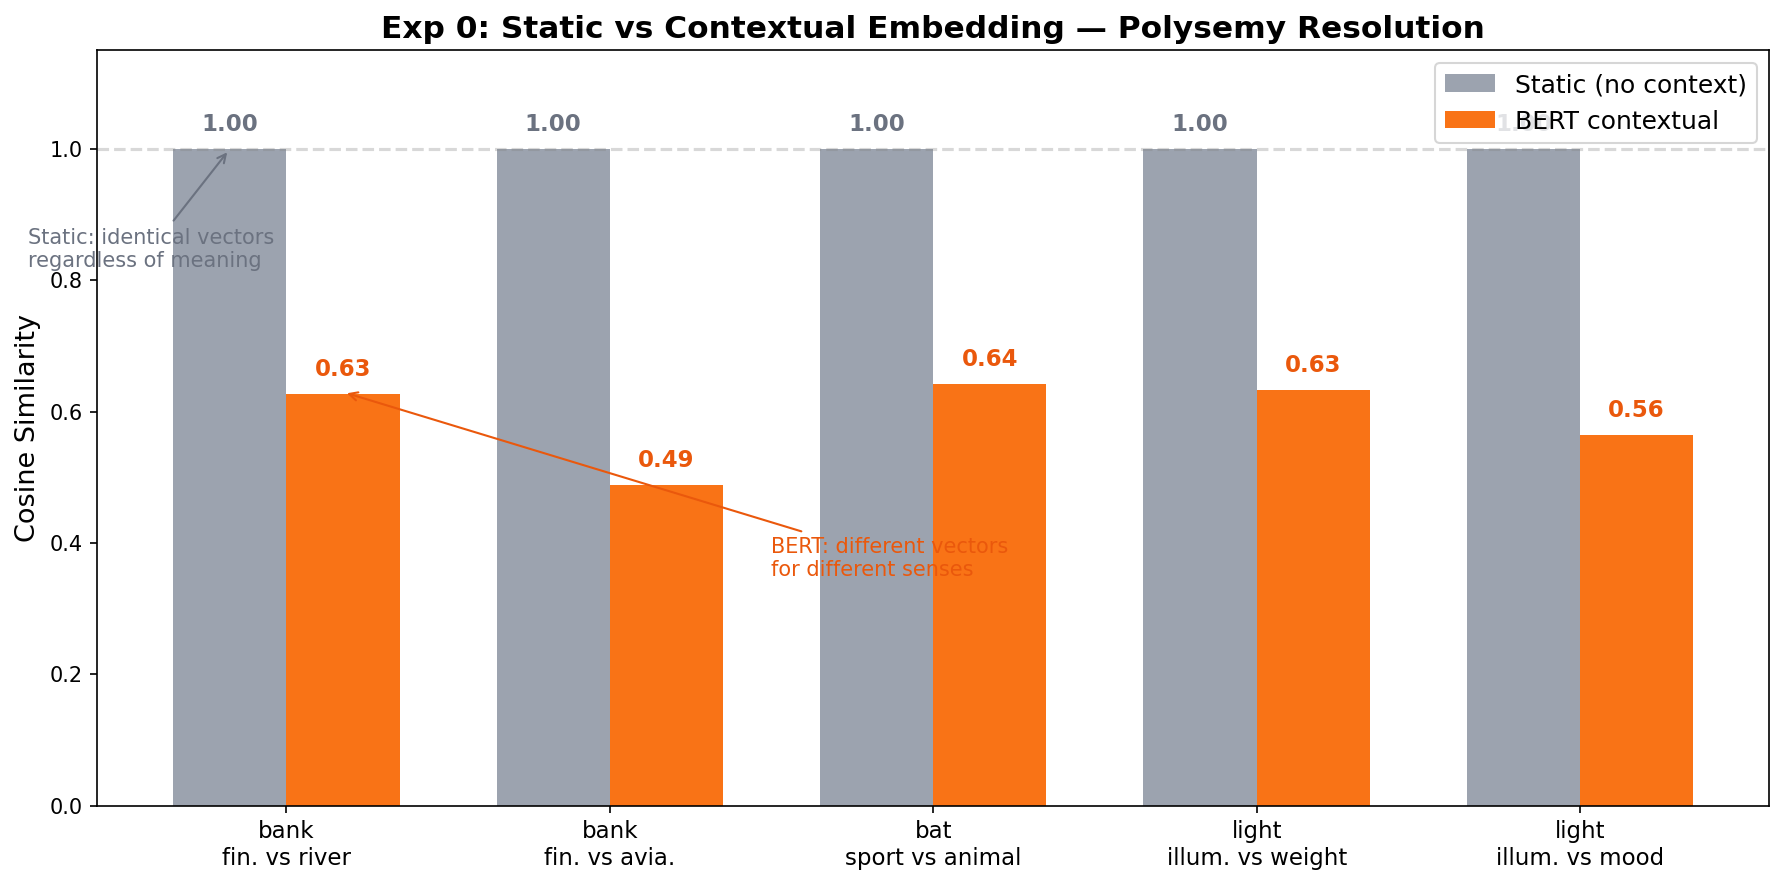
\includegraphics[width=0.95\textwidth]{labs/ch04/answers/figures/exp0_polysemy.png}
\caption{Static embeddings produce identical vectors for the same word regardless of context (cosine = 1.0). BERT's contextual embeddings produce clearly different vectors for different senses (cosine drops to 0.49--0.69), closing the loop from Lab~1 Exp~0.}
\label{fig:lab4-polysemy}
\end{figure}

\textbf{Core insight:} This directly answers Lab~1's open question. Static embeddings have a \emph{structural} polysemy limitation: one type, one vector. BERT solves it through bidirectional attention---each token's representation is a function of its complete sentence context. The loop from Lab~1 Exp~0 is closed.


\section{Exp 1: Frozen Probe on SST-2}

\textbf{Question:} Which encoder type captures more task-relevant information in its pretrained representations for sentence-level classification?

\textbf{Setup:} SST-2 sentiment classification (5000 train / 872 val). Freeze three encoders; train only a single linear classifier for 10 epochs. The only variable is the encoder type.

\begin{center}
\begin{tabular}{lcc}
\toprule
Encoder & Pooling & Val Accuracy \\
\midrule
Static (no context)       & mean of token embeddings & 70.4\% \\
DistilGPT2 (causal)       & last non-pad token       & 81.3\% \\
DistilBERT (bidirectional) & \texttt{[CLS]} token     & 81.1\% \\
\bottomrule
\end{tabular}
\end{center}

\begin{figure}[ht]
\centering
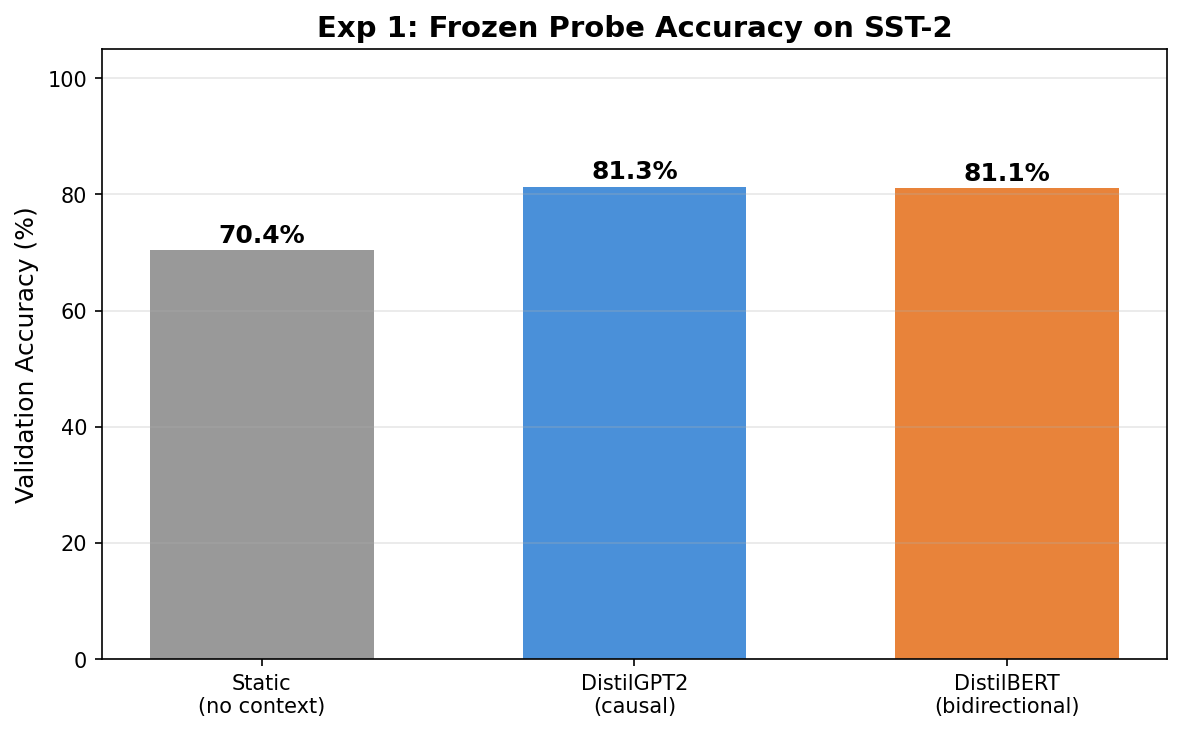
\includegraphics[width=0.75\textwidth]{labs/ch04/answers/figures/exp1_frozen_probe.png}
\caption{Frozen probe accuracy on SST-2. Static embeddings reach 70.4\%; both contextual models reach $\sim$81\% with no measurable gap between causal and bidirectional.}
\label{fig:lab4-frozen-probe}
\end{figure}

\textbf{Diagnosis:} The surprise: \textbf{GPT and BERT are essentially tied on sentence-level classification.} Both reach $\sim$81\%, with GPT marginally ahead. Context processing adds $\sim$10pp over static embeddings, but bidirectional vs.\ causal makes no difference here.

\textbf{Core insight:} SST-2 is a sentence-level task. GPT's last token has already processed the entire sentence left-to-right via causal attention. For the question ``is this sentence positive or negative?'', the last token's hidden state already encodes sufficient information. Bidirectional attention does not add measurable value for sentence-level aggregation. This is \emph{not} a failure of the experiment---it is one of the most important findings. It forces a precise question: \emph{where does the bidirectional advantage actually appear?} The next experiment answers it.


\section{Exp 2: Token-Level NER Probe (Key Experiment)}

\textbf{Question:} Does bidirectional context produce measurably better representations for token-level understanding tasks?

\textbf{Setup:} CoNLL-2003 Named Entity Recognition (5000 train / 1000 val, 9 labels). Full fine-tuning, 5 epochs, lr $= 2 \times 10^{-5}$. Both models use token classification heads. Subword alignment: only the first subword per word receives the NER label; continuation subwords are ignored.

\begin{center}
\begin{tabular}{lcc}
\toprule
Model & Token Accuracy & Macro Entity F1 \\
\midrule
DistilBERT (bidirectional) & \textbf{98.5\%} & \textbf{90.3\%} \\
DistilGPT2 (causal) & 93.7\% & 68.5\% \\
\midrule
Gap & +4.9pp & \textbf{+21.8pp} \\
\bottomrule
\end{tabular}
\end{center}

\textbf{Per-entity F1 breakdown:}

\begin{center}
\begin{tabular}{lccc}
\toprule
Entity type & DistilBERT & DistilGPT2 & Gap \\
\midrule
B-PER  & 99.0\% & 78.0\% & +21.0pp \\
B-ORG  & 90.6\% & 46.0\% & \textbf{+44.6pp} \\
B-LOC  & 95.6\% & 74.3\% & +21.3pp \\
B-MISC & 89.0\% & 50.0\% & \textbf{+39.0pp} \\
I-PER  & 98.5\% & 96.1\% & +2.4pp \\
I-ORG  & 86.1\% & 71.1\% & +15.0pp \\
I-LOC  & 84.9\% & 67.2\% & +17.7pp \\
I-MISC & 78.5\% & 65.0\% & +13.5pp \\
\bottomrule
\end{tabular}
\end{center}

\begin{figure}[ht]
\centering
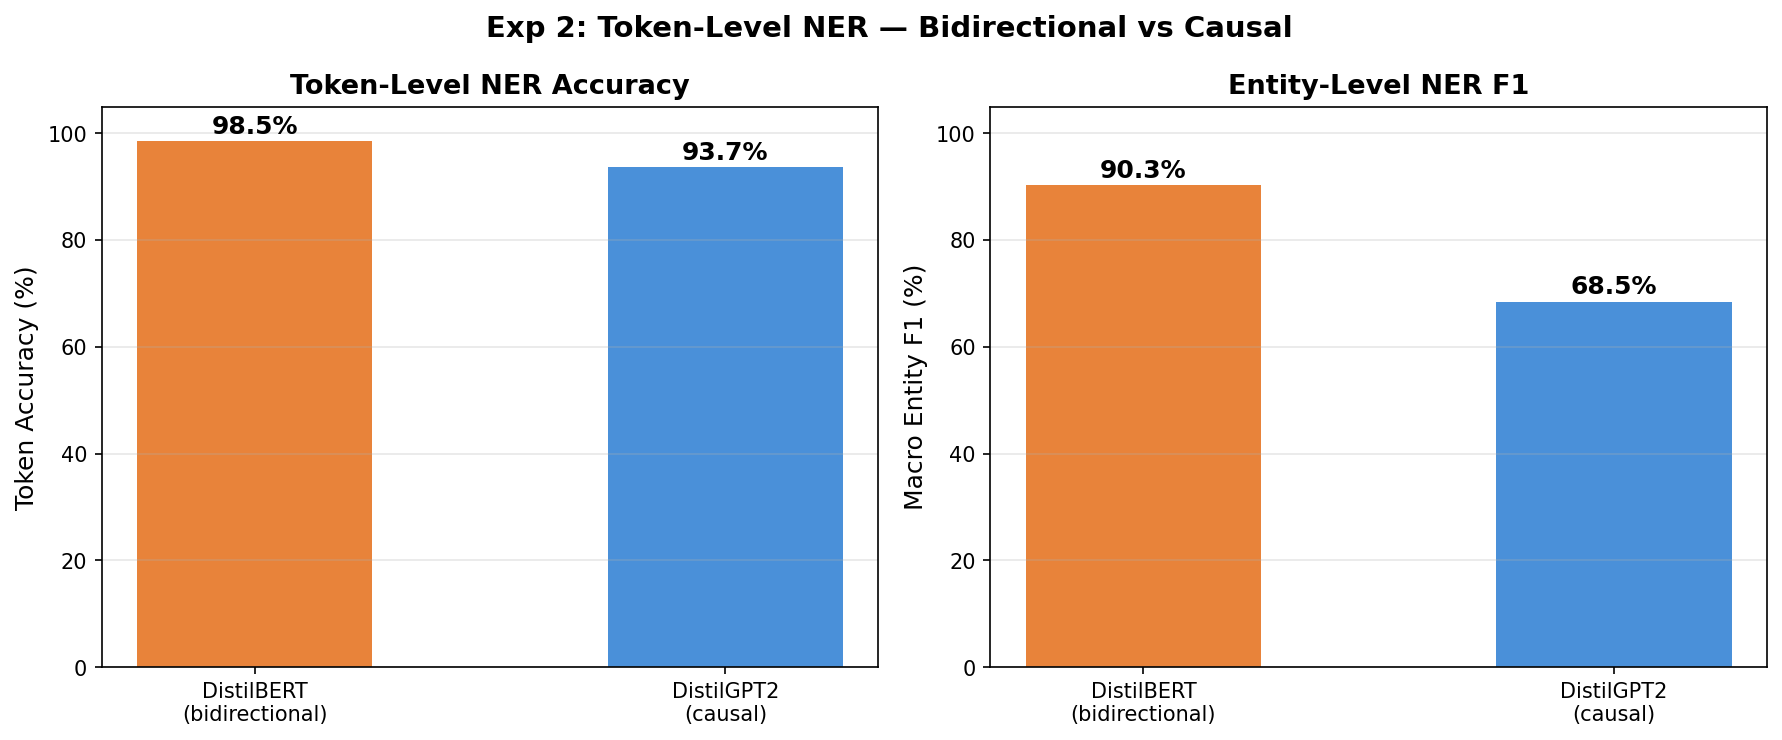
\includegraphics[width=0.85\textwidth]{labs/ch04/answers/figures/exp2_ner_comparison.png}
\caption{Token-level NER accuracy and entity F1: DistilBERT leads by 4.9pp on token accuracy and 21.8pp on entity F1---the largest effect in Lab~4.}
\label{fig:lab4-ner-comparison}
\end{figure}

\begin{figure}[ht]
\centering
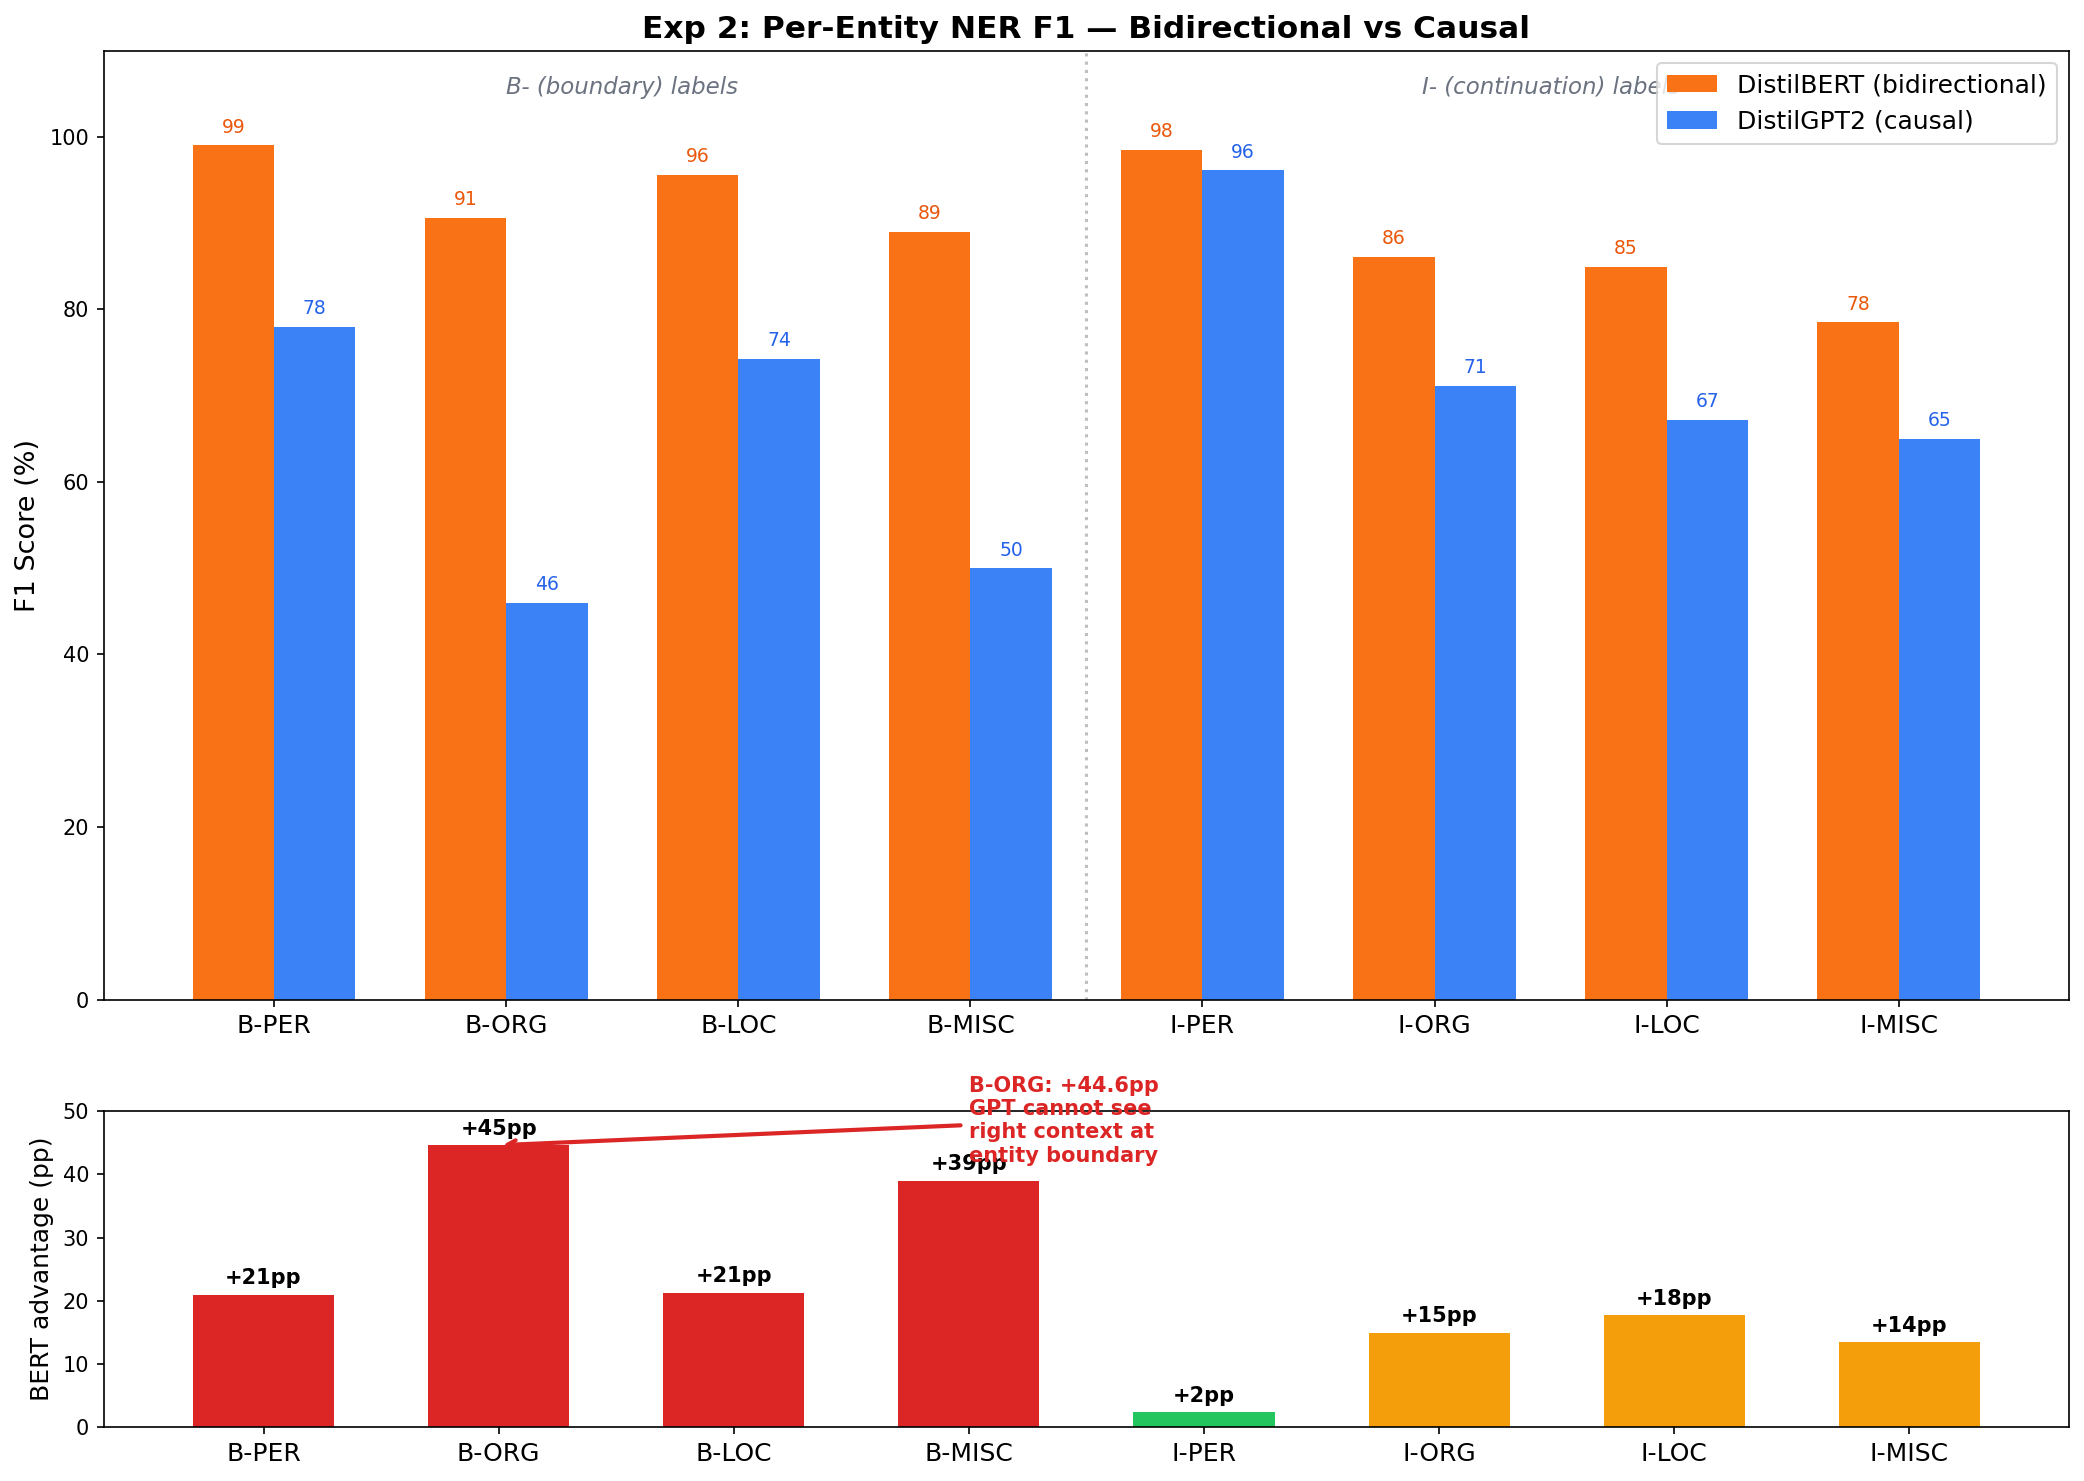
\includegraphics[width=0.95\textwidth]{labs/ch04/answers/figures/exp2_per_entity_f1.png}
\caption{Per-entity F1 breakdown. B- (boundary) labels show the largest BERT advantage (up to +44.6pp on B-ORG), while I- (continuation) labels show smaller gaps. GPT struggles most at entity boundaries because it cannot see right context to disambiguate.}
\label{fig:lab4-per-entity}
\end{figure}

\textbf{Diagnosis:} The entity F1 gap of \textbf{21.8 percentage points} is the largest effect in Lab~4. The pattern is striking: \textbf{B- (boundary) labels show the largest gaps} (up to +44.6pp on B-ORG), while \textbf{I- (continuation) labels show smaller gaps}. This makes perfect mechanical sense: when GPT encounters ``New,'' it does not know whether ``York Times'' follows---it cannot distinguish ``New York Times'' (B-ORG) from ``New ideas'' (O). By the time GPT processes a continuation token (I-ORG), it has already seen the B- token, so the gap shrinks.

\begin{figure}[ht]
\centering
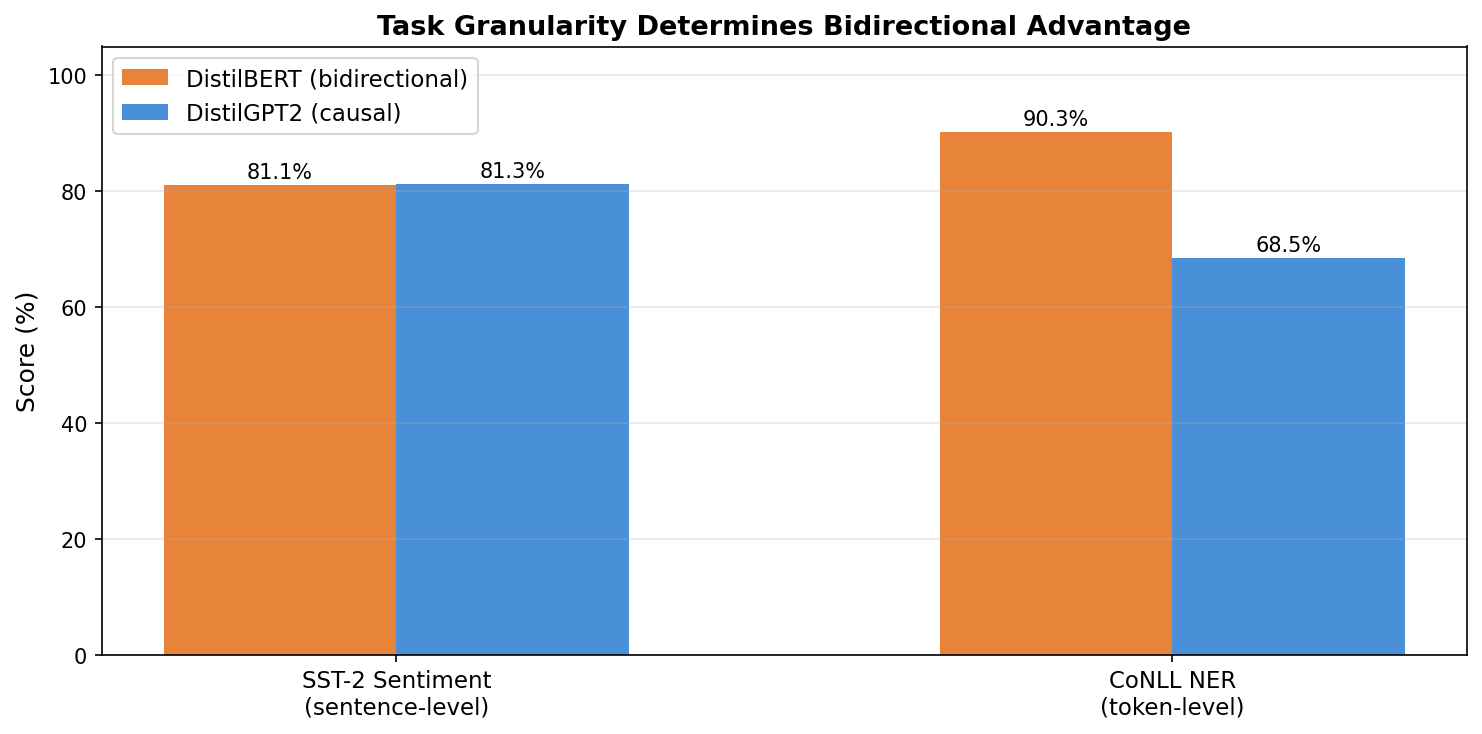
\includegraphics[width=0.8\textwidth]{labs/ch04/answers/figures/exp2_task_granularity.png}
\caption{Task granularity determines bidirectional advantage. On sentence-level SST-2, BERT and GPT are tied. On token-level NER, BERT leads by 21.8pp. The bidirectional advantage appears only when individual tokens need right-context.}
\label{fig:lab4-task-granularity}
\end{figure}

\textbf{Core insight:} Contrast this with Exp~1:

\begin{center}
\begin{tabular}{lccr}
\toprule
Task type & DistilBERT & DistilGPT2 & Gap \\
\midrule
SST-2 sentiment (sentence-level) & 81.1\% & 81.3\% & $\sim$0pp \\
CoNLL NER (token-level, entity F1) & \textbf{90.3\%} & \textbf{68.5\%} & \textbf{+21.8pp} \\
\bottomrule
\end{tabular}
\end{center}

\textbf{The bidirectional advantage is task-granularity dependent.} Sentence-level: causal is fine (the last token already saw everything). Token-level: bidirectional wins decisively (middle tokens need right-context that causal masking blocks). This is the central finding of Lab~4.


\section{Exp 3: SST-2 Fine-tune Comparison}

\textbf{Question:} Does full fine-tuning create a gap on sentence-level classification?

\textbf{Setup:} Fine-tune both models end-to-end on SST-2 (3 epochs, lr $= 2 \times 10^{-5}$, AdamW, batch size 16).

\begin{center}
\begin{tabular}{lccc}
\toprule
Model & Frozen (Exp 1) & Fine-tuned (Exp 3) & Improvement \\
\midrule
DistilBERT & 81.1\% & 87.0\% & +5.9pp \\
DistilGPT2 & 81.3\% & 87.4\% & +6.1pp \\
\midrule
Gap & $\sim$0pp & $\sim$0pp & no change \\
\bottomrule
\end{tabular}
\end{center}

\begin{figure}[ht]
\centering
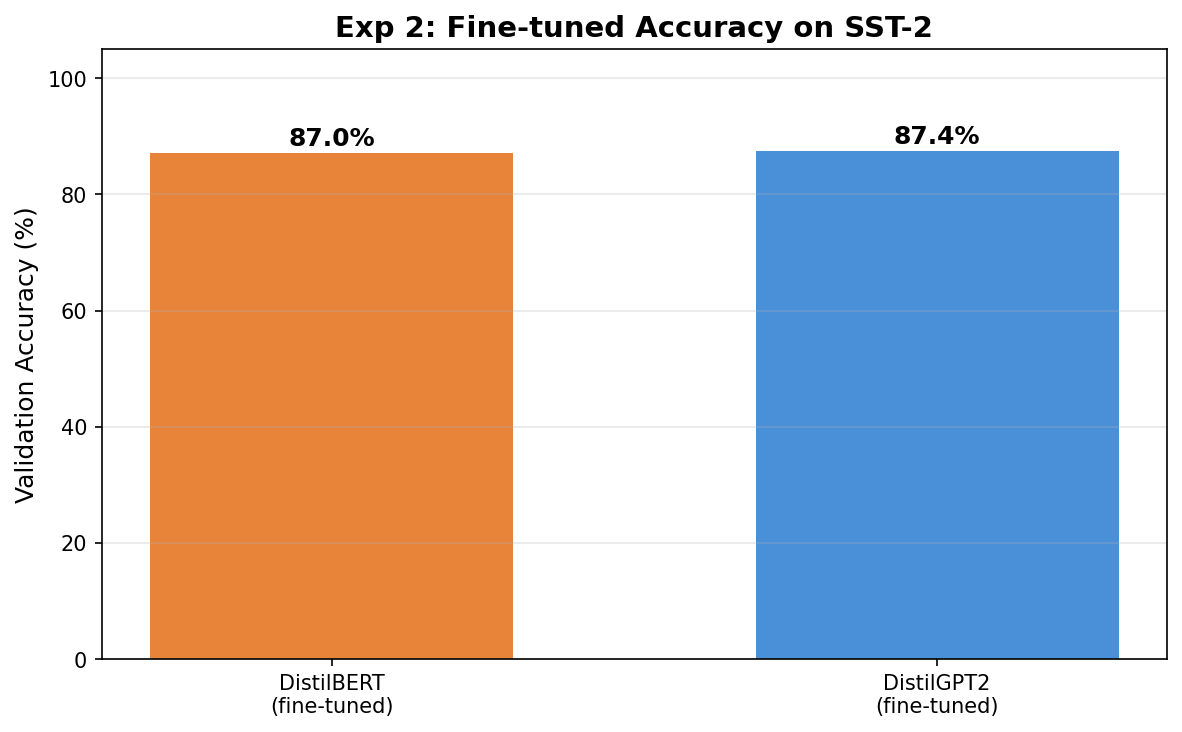
\includegraphics[width=0.65\textwidth]{labs/ch04/answers/figures/exp3_finetune.png}
\caption{Fine-tuned SST-2 accuracy. Both models improve by $\sim$6pp over frozen probing, but the gap remains near zero---confirming that sentence-level classification does not benefit from bidirectional attention.}
\label{fig:lab4-finetune}
\end{figure}

\textbf{Diagnosis:} Fine-tuning improves both models by $\sim$6pp, but the gap remains near zero. On sentence-level classification, GPT is genuinely as capable as BERT---both frozen and fine-tuned.

\textbf{Core insight:} The SST-2 parity is not a failure of the experiment. Combined with Exp~2's 21.8pp NER gap, it tells a precise story: GPT's causal mask is not a disability for sentence-level understanding, but it is a severe handicap for token-level understanding. BERT's advantage is \emph{specifically} about per-token representation quality, not about sentence-level aggregation.


\section{Exp 4: Generation Flip}

\textbf{Question:} If BERT is better at token-level understanding, what is GPT better at?

\textbf{Setup:} Pure inference, no training. Give both models the same prompts.

\textbf{GPT (autoregressive generation):}

\begin{quote}
\textbf{Prompt:} ``The movie was absolutely'' \\
\textbf{Output:} ``\ldots epic. I'd say that. But I love to see the story of Mark Twain. It's one of the best parts of his life\ldots''
\end{quote}

GPT produces fluent, multi-sentence continuations that naturally extend the prompt.

\textbf{BERT ([MASK] filling):}

\begin{center}
\begin{tabular}{lcc}
\toprule
Input & Top prediction & Score \\
\midrule
``The movie was absolutely {[MASK]}.'' & fantastic & 0.110 \\
``She felt {[MASK]} after hearing the news.'' & relieved & 0.075 \\
``The experiment was a complete {[MASK]}.'' & success & 0.462 \\
\bottomrule
\end{tabular}
\end{center}

BERT makes contextually appropriate predictions but can only fill one position at a time. Iterative mask filling produces grammatical output for short templates (``The movie was released on dvd by netflix'') but is fundamentally limited: each fill sees all positions, there is no left-to-right coherence, and output length cannot exceed the pre-specified mask count.

\textbf{Core insight:} Bidirectional attention prevents autoregressive generation. This is architectural, not a training deficiency. When users wanted AI that talks back, BERT could not comply---and this is the interface war it lost.


\section{Synthesis: Task Granularity Determines Architectural Advantage}

\begin{center}
\begin{tabular}{lccc}
\toprule
Task & DistilBERT & DistilGPT2 & Winner \\
\midrule
SST-2 frozen probe & 81.1\% & 81.3\% & Tied \\
SST-2 fine-tuned & 87.0\% & 87.4\% & Tied \\
NER entity F1 & \textbf{90.3\%} & 68.5\% & \textbf{BERT (+21.8pp)} \\
NER boundary (B-ORG) & \textbf{90.6\%} & 46.0\% & \textbf{BERT (+44.6pp)} \\
Text generation & {[MASK]} fill & Fluent text & \textbf{GPT} \\
Polysemy resolution & Resolved & --- & BERT \\
\bottomrule
\end{tabular}
\end{center}

Lab~4 refines Chapter~4's thesis to a precise claim:

\begin{quote}
\textbf{BERT wins when every token must independently encode full-context information. GPT wins when the task requires sequential generation. On sentence-level aggregation, they are equivalent.}
\end{quote}

This explains three facts about the current AI ecosystem:
\begin{enumerate}
\item BERT remains infrastructure for NER, retrieval, and reranking (token-level tasks).
\item GPT replaced BERT for chat, writing, and instruction following (generation tasks).
\item GPT can also do classification well (sentence-level tasks do not require bidirectional context).
\end{enumerate}

\textbf{Cross-lab connections:}
\begin{itemize}
\item \textbf{Lab~1 $\to$ Lab~4:} Lab~1 showed static embeddings cannot resolve polysemy; Lab~4 Exp~0 shows BERT solves it.
\item \textbf{Lab~3 $\to$ Lab~4:} Lab~3 diagnosed what makes a GPT trainable (residual stream, pre-norm). Lab~4 shows what GPT is good at (generation) and where BERT wins (token-level understanding). Same Transformer block, complementary strengths.
\item \textbf{The meta-lesson:} Capability is not determined by the Transformer block alone. It emerges from the interaction of architecture, mask, and training objective. This is the central lesson of Part~I.
\end{itemize}
